% Created by tikzDevice version 0.12.3.1 on 2022-02-28 16:48:41
% !TEX encoding = UTF-8 Unicode
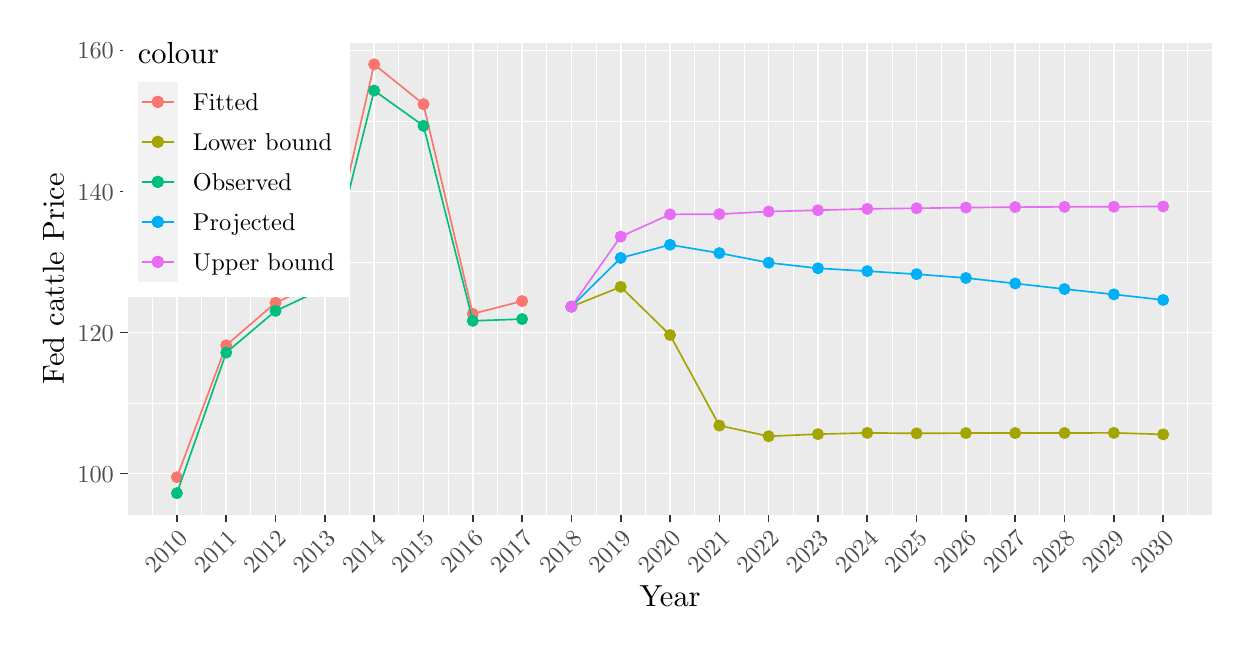
\begin{tikzpicture}[x=1pt,y=1pt]
\definecolor{fillColor}{RGB}{255,255,255}
\path[use as bounding box,fill=fillColor,fill opacity=0.00] (0,0) rectangle (433.62,216.81);
\begin{scope}
\path[clip] (  0.00,  0.00) rectangle (433.62,216.81);
\definecolor{drawColor}{RGB}{255,255,255}
\definecolor{fillColor}{RGB}{255,255,255}

\path[draw=drawColor,line width= 0.6pt,line join=round,line cap=round,fill=fillColor] (  0.00,  0.00) rectangle (433.62,216.81);
\end{scope}
\begin{scope}
\path[clip] ( 36.11, 40.85) rectangle (428.12,211.31);
\definecolor{fillColor}{gray}{0.92}

\path[fill=fillColor] ( 36.11, 40.85) rectangle (428.12,211.31);
\definecolor{drawColor}{RGB}{255,255,255}

\path[draw=drawColor,line width= 0.3pt,line join=round] ( 36.11, 81.14) --
	(428.12, 81.14);

\path[draw=drawColor,line width= 0.3pt,line join=round] ( 36.11,132.09) --
	(428.12,132.09);

\path[draw=drawColor,line width= 0.3pt,line join=round] ( 36.11,183.05) --
	(428.12,183.05);

\path[draw=drawColor,line width= 0.3pt,line join=round] ( 36.11, 40.85) --
	( 36.11,211.31);

\path[draw=drawColor,line width= 0.3pt,line join=round] ( 45.02, 40.85) --
	( 45.02,211.31);

\path[draw=drawColor,line width= 0.3pt,line join=round] ( 62.84, 40.85) --
	( 62.84,211.31);

\path[draw=drawColor,line width= 0.3pt,line join=round] ( 80.66, 40.85) --
	( 80.66,211.31);

\path[draw=drawColor,line width= 0.3pt,line join=round] ( 98.48, 40.85) --
	( 98.48,211.31);

\path[draw=drawColor,line width= 0.3pt,line join=round] (116.29, 40.85) --
	(116.29,211.31);

\path[draw=drawColor,line width= 0.3pt,line join=round] (134.11, 40.85) --
	(134.11,211.31);

\path[draw=drawColor,line width= 0.3pt,line join=round] (151.93, 40.85) --
	(151.93,211.31);

\path[draw=drawColor,line width= 0.3pt,line join=round] (169.75, 40.85) --
	(169.75,211.31);

\path[draw=drawColor,line width= 0.3pt,line join=round] (187.57, 40.85) --
	(187.57,211.31);

\path[draw=drawColor,line width= 0.3pt,line join=round] (205.39, 40.85) --
	(205.39,211.31);

\path[draw=drawColor,line width= 0.3pt,line join=round] (223.21, 40.85) --
	(223.21,211.31);

\path[draw=drawColor,line width= 0.3pt,line join=round] (241.02, 40.85) --
	(241.02,211.31);

\path[draw=drawColor,line width= 0.3pt,line join=round] (258.84, 40.85) --
	(258.84,211.31);

\path[draw=drawColor,line width= 0.3pt,line join=round] (276.66, 40.85) --
	(276.66,211.31);

\path[draw=drawColor,line width= 0.3pt,line join=round] (294.48, 40.85) --
	(294.48,211.31);

\path[draw=drawColor,line width= 0.3pt,line join=round] (312.30, 40.85) --
	(312.30,211.31);

\path[draw=drawColor,line width= 0.3pt,line join=round] (330.12, 40.85) --
	(330.12,211.31);

\path[draw=drawColor,line width= 0.3pt,line join=round] (347.94, 40.85) --
	(347.94,211.31);

\path[draw=drawColor,line width= 0.3pt,line join=round] (365.75, 40.85) --
	(365.75,211.31);

\path[draw=drawColor,line width= 0.3pt,line join=round] (383.57, 40.85) --
	(383.57,211.31);

\path[draw=drawColor,line width= 0.3pt,line join=round] (401.39, 40.85) --
	(401.39,211.31);

\path[draw=drawColor,line width= 0.3pt,line join=round] (419.21, 40.85) --
	(419.21,211.31);

\path[draw=drawColor,line width= 0.3pt,line join=round] (428.12, 40.85) --
	(428.12,211.31);

\path[draw=drawColor,line width= 0.6pt,line join=round] ( 36.11, 55.66) --
	(428.12, 55.66);

\path[draw=drawColor,line width= 0.6pt,line join=round] ( 36.11,106.62) --
	(428.12,106.62);

\path[draw=drawColor,line width= 0.6pt,line join=round] ( 36.11,157.57) --
	(428.12,157.57);

\path[draw=drawColor,line width= 0.6pt,line join=round] ( 36.11,208.53) --
	(428.12,208.53);

\path[draw=drawColor,line width= 0.6pt,line join=round] ( 53.93, 40.85) --
	( 53.93,211.31);

\path[draw=drawColor,line width= 0.6pt,line join=round] ( 71.75, 40.85) --
	( 71.75,211.31);

\path[draw=drawColor,line width= 0.6pt,line join=round] ( 89.57, 40.85) --
	( 89.57,211.31);

\path[draw=drawColor,line width= 0.6pt,line join=round] (107.39, 40.85) --
	(107.39,211.31);

\path[draw=drawColor,line width= 0.6pt,line join=round] (125.20, 40.85) --
	(125.20,211.31);

\path[draw=drawColor,line width= 0.6pt,line join=round] (143.02, 40.85) --
	(143.02,211.31);

\path[draw=drawColor,line width= 0.6pt,line join=round] (160.84, 40.85) --
	(160.84,211.31);

\path[draw=drawColor,line width= 0.6pt,line join=round] (178.66, 40.85) --
	(178.66,211.31);

\path[draw=drawColor,line width= 0.6pt,line join=round] (196.48, 40.85) --
	(196.48,211.31);

\path[draw=drawColor,line width= 0.6pt,line join=round] (214.30, 40.85) --
	(214.30,211.31);

\path[draw=drawColor,line width= 0.6pt,line join=round] (232.12, 40.85) --
	(232.12,211.31);

\path[draw=drawColor,line width= 0.6pt,line join=round] (249.93, 40.85) --
	(249.93,211.31);

\path[draw=drawColor,line width= 0.6pt,line join=round] (267.75, 40.85) --
	(267.75,211.31);

\path[draw=drawColor,line width= 0.6pt,line join=round] (285.57, 40.85) --
	(285.57,211.31);

\path[draw=drawColor,line width= 0.6pt,line join=round] (303.39, 40.85) --
	(303.39,211.31);

\path[draw=drawColor,line width= 0.6pt,line join=round] (321.21, 40.85) --
	(321.21,211.31);

\path[draw=drawColor,line width= 0.6pt,line join=round] (339.03, 40.85) --
	(339.03,211.31);

\path[draw=drawColor,line width= 0.6pt,line join=round] (356.85, 40.85) --
	(356.85,211.31);

\path[draw=drawColor,line width= 0.6pt,line join=round] (374.66, 40.85) --
	(374.66,211.31);

\path[draw=drawColor,line width= 0.6pt,line join=round] (392.48, 40.85) --
	(392.48,211.31);

\path[draw=drawColor,line width= 0.6pt,line join=round] (410.30, 40.85) --
	(410.30,211.31);
\definecolor{drawColor}{RGB}{248,118,109}

\path[draw=drawColor,line width= 0.6pt,line join=round] ( 53.93, 54.36) --
	( 71.75,102.05) --
	( 89.57,117.42) --
	(107.39,125.57) --
	(125.20,203.56) --
	(143.02,189.17) --
	(160.84,113.42) --
	(178.66,118.00);
\definecolor{fillColor}{RGB}{248,118,109}

\path[draw=drawColor,line width= 0.4pt,line join=round,line cap=round,fill=fillColor] ( 53.93, 54.36) circle (  1.96);

\path[draw=drawColor,line width= 0.4pt,line join=round,line cap=round,fill=fillColor] ( 71.75,102.05) circle (  1.96);

\path[draw=drawColor,line width= 0.4pt,line join=round,line cap=round,fill=fillColor] ( 89.57,117.42) circle (  1.96);

\path[draw=drawColor,line width= 0.4pt,line join=round,line cap=round,fill=fillColor] (107.39,125.57) circle (  1.96);

\path[draw=drawColor,line width= 0.4pt,line join=round,line cap=round,fill=fillColor] (125.20,203.56) circle (  1.96);

\path[draw=drawColor,line width= 0.4pt,line join=round,line cap=round,fill=fillColor] (143.02,189.17) circle (  1.96);

\path[draw=drawColor,line width= 0.4pt,line join=round,line cap=round,fill=fillColor] (160.84,113.42) circle (  1.96);

\path[draw=drawColor,line width= 0.4pt,line join=round,line cap=round,fill=fillColor] (178.66,118.00) circle (  1.96);
\definecolor{drawColor}{RGB}{0,191,125}

\path[draw=drawColor,line width= 0.6pt,line join=round] ( 53.93, 48.60) --
	( 71.75, 99.40) --
	( 89.57,114.46) --
	(107.39,122.74) --
	(125.20,194.08) --
	(143.02,181.34) --
	(160.84,110.87) --
	(178.66,111.51);
\definecolor{fillColor}{RGB}{0,191,125}

\path[draw=drawColor,line width= 0.4pt,line join=round,line cap=round,fill=fillColor] ( 53.93, 48.60) circle (  1.96);

\path[draw=drawColor,line width= 0.4pt,line join=round,line cap=round,fill=fillColor] ( 71.75, 99.40) circle (  1.96);

\path[draw=drawColor,line width= 0.4pt,line join=round,line cap=round,fill=fillColor] ( 89.57,114.46) circle (  1.96);

\path[draw=drawColor,line width= 0.4pt,line join=round,line cap=round,fill=fillColor] (107.39,122.74) circle (  1.96);

\path[draw=drawColor,line width= 0.4pt,line join=round,line cap=round,fill=fillColor] (125.20,194.08) circle (  1.96);

\path[draw=drawColor,line width= 0.4pt,line join=round,line cap=round,fill=fillColor] (143.02,181.34) circle (  1.96);

\path[draw=drawColor,line width= 0.4pt,line join=round,line cap=round,fill=fillColor] (160.84,110.87) circle (  1.96);

\path[draw=drawColor,line width= 0.4pt,line join=round,line cap=round,fill=fillColor] (178.66,111.51) circle (  1.96);
\definecolor{drawColor}{RGB}{163,165,0}

\path[draw=drawColor,line width= 0.6pt,line join=round] (196.48,116.00) --
	(214.30,123.15) --
	(232.12,105.74) --
	(249.93, 73.04) --
	(267.75, 69.17) --
	(285.57, 69.93) --
	(303.39, 70.38) --
	(321.21, 70.22) --
	(339.03, 70.32) --
	(356.85, 70.33) --
	(374.66, 70.35) --
	(392.48, 70.39) --
	(410.30, 69.85);
\definecolor{fillColor}{RGB}{163,165,0}

\path[draw=drawColor,line width= 0.4pt,line join=round,line cap=round,fill=fillColor] (196.48,116.00) circle (  1.96);

\path[draw=drawColor,line width= 0.4pt,line join=round,line cap=round,fill=fillColor] (214.30,123.15) circle (  1.96);

\path[draw=drawColor,line width= 0.4pt,line join=round,line cap=round,fill=fillColor] (232.12,105.74) circle (  1.96);

\path[draw=drawColor,line width= 0.4pt,line join=round,line cap=round,fill=fillColor] (249.93, 73.04) circle (  1.96);

\path[draw=drawColor,line width= 0.4pt,line join=round,line cap=round,fill=fillColor] (267.75, 69.17) circle (  1.96);

\path[draw=drawColor,line width= 0.4pt,line join=round,line cap=round,fill=fillColor] (285.57, 69.93) circle (  1.96);

\path[draw=drawColor,line width= 0.4pt,line join=round,line cap=round,fill=fillColor] (303.39, 70.38) circle (  1.96);

\path[draw=drawColor,line width= 0.4pt,line join=round,line cap=round,fill=fillColor] (321.21, 70.22) circle (  1.96);

\path[draw=drawColor,line width= 0.4pt,line join=round,line cap=round,fill=fillColor] (339.03, 70.32) circle (  1.96);

\path[draw=drawColor,line width= 0.4pt,line join=round,line cap=round,fill=fillColor] (356.85, 70.33) circle (  1.96);

\path[draw=drawColor,line width= 0.4pt,line join=round,line cap=round,fill=fillColor] (374.66, 70.35) circle (  1.96);

\path[draw=drawColor,line width= 0.4pt,line join=round,line cap=round,fill=fillColor] (392.48, 70.39) circle (  1.96);

\path[draw=drawColor,line width= 0.4pt,line join=round,line cap=round,fill=fillColor] (410.30, 69.85) circle (  1.96);
\definecolor{drawColor}{RGB}{0,176,246}

\path[draw=drawColor,line width= 0.6pt,line join=round] (196.48,116.00) --
	(214.30,133.60) --
	(232.12,138.35) --
	(249.93,135.35) --
	(267.75,131.88) --
	(285.57,129.86) --
	(303.39,128.83) --
	(321.21,127.73) --
	(339.03,126.36) --
	(356.85,124.37) --
	(374.66,122.36) --
	(392.48,120.43) --
	(410.30,118.43);
\definecolor{fillColor}{RGB}{0,176,246}

\path[draw=drawColor,line width= 0.4pt,line join=round,line cap=round,fill=fillColor] (196.48,116.00) circle (  1.96);

\path[draw=drawColor,line width= 0.4pt,line join=round,line cap=round,fill=fillColor] (214.30,133.60) circle (  1.96);

\path[draw=drawColor,line width= 0.4pt,line join=round,line cap=round,fill=fillColor] (232.12,138.35) circle (  1.96);

\path[draw=drawColor,line width= 0.4pt,line join=round,line cap=round,fill=fillColor] (249.93,135.35) circle (  1.96);

\path[draw=drawColor,line width= 0.4pt,line join=round,line cap=round,fill=fillColor] (267.75,131.88) circle (  1.96);

\path[draw=drawColor,line width= 0.4pt,line join=round,line cap=round,fill=fillColor] (285.57,129.86) circle (  1.96);

\path[draw=drawColor,line width= 0.4pt,line join=round,line cap=round,fill=fillColor] (303.39,128.83) circle (  1.96);

\path[draw=drawColor,line width= 0.4pt,line join=round,line cap=round,fill=fillColor] (321.21,127.73) circle (  1.96);

\path[draw=drawColor,line width= 0.4pt,line join=round,line cap=round,fill=fillColor] (339.03,126.36) circle (  1.96);

\path[draw=drawColor,line width= 0.4pt,line join=round,line cap=round,fill=fillColor] (356.85,124.37) circle (  1.96);

\path[draw=drawColor,line width= 0.4pt,line join=round,line cap=round,fill=fillColor] (374.66,122.36) circle (  1.96);

\path[draw=drawColor,line width= 0.4pt,line join=round,line cap=round,fill=fillColor] (392.48,120.43) circle (  1.96);

\path[draw=drawColor,line width= 0.4pt,line join=round,line cap=round,fill=fillColor] (410.30,118.43) circle (  1.96);
\definecolor{drawColor}{RGB}{231,107,243}

\path[draw=drawColor,line width= 0.6pt,line join=round] (196.48,116.00) --
	(214.30,141.32) --
	(232.12,149.34) --
	(249.93,149.43) --
	(267.75,150.37) --
	(285.57,150.84) --
	(303.39,151.34) --
	(321.21,151.55) --
	(339.03,151.80) --
	(356.85,151.96) --
	(374.66,152.06) --
	(392.48,152.09) --
	(410.30,152.21);
\definecolor{fillColor}{RGB}{231,107,243}

\path[draw=drawColor,line width= 0.4pt,line join=round,line cap=round,fill=fillColor] (196.48,116.00) circle (  1.96);

\path[draw=drawColor,line width= 0.4pt,line join=round,line cap=round,fill=fillColor] (214.30,141.32) circle (  1.96);

\path[draw=drawColor,line width= 0.4pt,line join=round,line cap=round,fill=fillColor] (232.12,149.34) circle (  1.96);

\path[draw=drawColor,line width= 0.4pt,line join=round,line cap=round,fill=fillColor] (249.93,149.43) circle (  1.96);

\path[draw=drawColor,line width= 0.4pt,line join=round,line cap=round,fill=fillColor] (267.75,150.37) circle (  1.96);

\path[draw=drawColor,line width= 0.4pt,line join=round,line cap=round,fill=fillColor] (285.57,150.84) circle (  1.96);

\path[draw=drawColor,line width= 0.4pt,line join=round,line cap=round,fill=fillColor] (303.39,151.34) circle (  1.96);

\path[draw=drawColor,line width= 0.4pt,line join=round,line cap=round,fill=fillColor] (321.21,151.55) circle (  1.96);

\path[draw=drawColor,line width= 0.4pt,line join=round,line cap=round,fill=fillColor] (339.03,151.80) circle (  1.96);

\path[draw=drawColor,line width= 0.4pt,line join=round,line cap=round,fill=fillColor] (356.85,151.96) circle (  1.96);

\path[draw=drawColor,line width= 0.4pt,line join=round,line cap=round,fill=fillColor] (374.66,152.06) circle (  1.96);

\path[draw=drawColor,line width= 0.4pt,line join=round,line cap=round,fill=fillColor] (392.48,152.09) circle (  1.96);

\path[draw=drawColor,line width= 0.4pt,line join=round,line cap=round,fill=fillColor] (410.30,152.21) circle (  1.96);
\end{scope}
\begin{scope}
\path[clip] (  0.00,  0.00) rectangle (433.62,216.81);
\definecolor{drawColor}{gray}{0.30}

\node[text=drawColor,anchor=base east,inner sep=0pt, outer sep=0pt, scale=  0.88] at ( 31.16, 52.63) {100};

\node[text=drawColor,anchor=base east,inner sep=0pt, outer sep=0pt, scale=  0.88] at ( 31.16,103.58) {120};

\node[text=drawColor,anchor=base east,inner sep=0pt, outer sep=0pt, scale=  0.88] at ( 31.16,154.54) {140};

\node[text=drawColor,anchor=base east,inner sep=0pt, outer sep=0pt, scale=  0.88] at ( 31.16,205.50) {160};
\end{scope}
\begin{scope}
\path[clip] (  0.00,  0.00) rectangle (433.62,216.81);
\definecolor{drawColor}{gray}{0.20}

\path[draw=drawColor,line width= 0.6pt,line join=round] ( 33.36, 55.66) --
	( 36.11, 55.66);

\path[draw=drawColor,line width= 0.6pt,line join=round] ( 33.36,106.62) --
	( 36.11,106.62);

\path[draw=drawColor,line width= 0.6pt,line join=round] ( 33.36,157.57) --
	( 36.11,157.57);

\path[draw=drawColor,line width= 0.6pt,line join=round] ( 33.36,208.53) --
	( 36.11,208.53);
\end{scope}
\begin{scope}
\path[clip] (  0.00,  0.00) rectangle (433.62,216.81);
\definecolor{drawColor}{gray}{0.20}

\path[draw=drawColor,line width= 0.6pt,line join=round] ( 53.93, 38.10) --
	( 53.93, 40.85);

\path[draw=drawColor,line width= 0.6pt,line join=round] ( 71.75, 38.10) --
	( 71.75, 40.85);

\path[draw=drawColor,line width= 0.6pt,line join=round] ( 89.57, 38.10) --
	( 89.57, 40.85);

\path[draw=drawColor,line width= 0.6pt,line join=round] (107.39, 38.10) --
	(107.39, 40.85);

\path[draw=drawColor,line width= 0.6pt,line join=round] (125.20, 38.10) --
	(125.20, 40.85);

\path[draw=drawColor,line width= 0.6pt,line join=round] (143.02, 38.10) --
	(143.02, 40.85);

\path[draw=drawColor,line width= 0.6pt,line join=round] (160.84, 38.10) --
	(160.84, 40.85);

\path[draw=drawColor,line width= 0.6pt,line join=round] (178.66, 38.10) --
	(178.66, 40.85);

\path[draw=drawColor,line width= 0.6pt,line join=round] (196.48, 38.10) --
	(196.48, 40.85);

\path[draw=drawColor,line width= 0.6pt,line join=round] (214.30, 38.10) --
	(214.30, 40.85);

\path[draw=drawColor,line width= 0.6pt,line join=round] (232.12, 38.10) --
	(232.12, 40.85);

\path[draw=drawColor,line width= 0.6pt,line join=round] (249.93, 38.10) --
	(249.93, 40.85);

\path[draw=drawColor,line width= 0.6pt,line join=round] (267.75, 38.10) --
	(267.75, 40.85);

\path[draw=drawColor,line width= 0.6pt,line join=round] (285.57, 38.10) --
	(285.57, 40.85);

\path[draw=drawColor,line width= 0.6pt,line join=round] (303.39, 38.10) --
	(303.39, 40.85);

\path[draw=drawColor,line width= 0.6pt,line join=round] (321.21, 38.10) --
	(321.21, 40.85);

\path[draw=drawColor,line width= 0.6pt,line join=round] (339.03, 38.10) --
	(339.03, 40.85);

\path[draw=drawColor,line width= 0.6pt,line join=round] (356.85, 38.10) --
	(356.85, 40.85);

\path[draw=drawColor,line width= 0.6pt,line join=round] (374.66, 38.10) --
	(374.66, 40.85);

\path[draw=drawColor,line width= 0.6pt,line join=round] (392.48, 38.10) --
	(392.48, 40.85);

\path[draw=drawColor,line width= 0.6pt,line join=round] (410.30, 38.10) --
	(410.30, 40.85);
\end{scope}
\begin{scope}
\path[clip] (  0.00,  0.00) rectangle (433.62,216.81);
\definecolor{drawColor}{gray}{0.30}

\node[text=drawColor,rotate= 45.00,anchor=base east,inner sep=0pt, outer sep=0pt, scale=  0.88] at ( 58.22, 31.62) {2010};

\node[text=drawColor,rotate= 45.00,anchor=base east,inner sep=0pt, outer sep=0pt, scale=  0.88] at ( 76.03, 31.62) {2011};

\node[text=drawColor,rotate= 45.00,anchor=base east,inner sep=0pt, outer sep=0pt, scale=  0.88] at ( 93.85, 31.62) {2012};

\node[text=drawColor,rotate= 45.00,anchor=base east,inner sep=0pt, outer sep=0pt, scale=  0.88] at (111.67, 31.62) {2013};

\node[text=drawColor,rotate= 45.00,anchor=base east,inner sep=0pt, outer sep=0pt, scale=  0.88] at (129.49, 31.62) {2014};

\node[text=drawColor,rotate= 45.00,anchor=base east,inner sep=0pt, outer sep=0pt, scale=  0.88] at (147.31, 31.62) {2015};

\node[text=drawColor,rotate= 45.00,anchor=base east,inner sep=0pt, outer sep=0pt, scale=  0.88] at (165.13, 31.62) {2016};

\node[text=drawColor,rotate= 45.00,anchor=base east,inner sep=0pt, outer sep=0pt, scale=  0.88] at (182.95, 31.62) {2017};

\node[text=drawColor,rotate= 45.00,anchor=base east,inner sep=0pt, outer sep=0pt, scale=  0.88] at (200.76, 31.62) {2018};

\node[text=drawColor,rotate= 45.00,anchor=base east,inner sep=0pt, outer sep=0pt, scale=  0.88] at (218.58, 31.62) {2019};

\node[text=drawColor,rotate= 45.00,anchor=base east,inner sep=0pt, outer sep=0pt, scale=  0.88] at (236.40, 31.62) {2020};

\node[text=drawColor,rotate= 45.00,anchor=base east,inner sep=0pt, outer sep=0pt, scale=  0.88] at (254.22, 31.62) {2021};

\node[text=drawColor,rotate= 45.00,anchor=base east,inner sep=0pt, outer sep=0pt, scale=  0.88] at (272.04, 31.62) {2022};

\node[text=drawColor,rotate= 45.00,anchor=base east,inner sep=0pt, outer sep=0pt, scale=  0.88] at (289.86, 31.62) {2023};

\node[text=drawColor,rotate= 45.00,anchor=base east,inner sep=0pt, outer sep=0pt, scale=  0.88] at (307.68, 31.62) {2024};

\node[text=drawColor,rotate= 45.00,anchor=base east,inner sep=0pt, outer sep=0pt, scale=  0.88] at (325.49, 31.62) {2025};

\node[text=drawColor,rotate= 45.00,anchor=base east,inner sep=0pt, outer sep=0pt, scale=  0.88] at (343.31, 31.62) {2026};

\node[text=drawColor,rotate= 45.00,anchor=base east,inner sep=0pt, outer sep=0pt, scale=  0.88] at (361.13, 31.62) {2027};

\node[text=drawColor,rotate= 45.00,anchor=base east,inner sep=0pt, outer sep=0pt, scale=  0.88] at (378.95, 31.62) {2028};

\node[text=drawColor,rotate= 45.00,anchor=base east,inner sep=0pt, outer sep=0pt, scale=  0.88] at (396.77, 31.62) {2029};

\node[text=drawColor,rotate= 45.00,anchor=base east,inner sep=0pt, outer sep=0pt, scale=  0.88] at (414.59, 31.62) {2030};
\end{scope}
\begin{scope}
\path[clip] (  0.00,  0.00) rectangle (433.62,216.81);
\definecolor{drawColor}{RGB}{0,0,0}

\node[text=drawColor,anchor=base,inner sep=0pt, outer sep=0pt, scale=  1.10] at (232.12,  7.64) {Year};
\end{scope}
\begin{scope}
\path[clip] (  0.00,  0.00) rectangle (433.62,216.81);
\definecolor{drawColor}{RGB}{0,0,0}

\node[text=drawColor,rotate= 90.00,anchor=base,inner sep=0pt, outer sep=0pt, scale=  1.10] at ( 13.08,126.08) {Fed cattle Price};
\end{scope}
\begin{scope}
\path[clip] (  0.00,  0.00) rectangle (433.62,216.81);
\definecolor{fillColor}{RGB}{255,255,255}

\path[fill=fillColor] ( 34.28,119.45) rectangle (116.34,217.94);
\end{scope}
\begin{scope}
\path[clip] (  0.00,  0.00) rectangle (433.62,216.81);
\definecolor{drawColor}{RGB}{0,0,0}

\node[text=drawColor,anchor=base west,inner sep=0pt, outer sep=0pt, scale=  1.10] at ( 39.78,203.79) {colour};
\end{scope}
\begin{scope}
\path[clip] (  0.00,  0.00) rectangle (433.62,216.81);
\definecolor{fillColor}{gray}{0.95}

\path[fill=fillColor] ( 39.78,182.77) rectangle ( 54.24,197.22);
\end{scope}
\begin{scope}
\path[clip] (  0.00,  0.00) rectangle (433.62,216.81);
\definecolor{drawColor}{RGB}{248,118,109}

\path[draw=drawColor,line width= 0.6pt,line join=round] ( 41.23,190.00) -- ( 52.79,190.00);
\end{scope}
\begin{scope}
\path[clip] (  0.00,  0.00) rectangle (433.62,216.81);
\definecolor{drawColor}{RGB}{248,118,109}
\definecolor{fillColor}{RGB}{248,118,109}

\path[draw=drawColor,line width= 0.4pt,line join=round,line cap=round,fill=fillColor] ( 47.01,190.00) circle (  1.96);
\end{scope}
\begin{scope}
\path[clip] (  0.00,  0.00) rectangle (433.62,216.81);
\definecolor{drawColor}{RGB}{248,118,109}

\path[draw=drawColor,line width= 0.6pt,line join=round] ( 41.23,190.00) -- ( 52.79,190.00);
\end{scope}
\begin{scope}
\path[clip] (  0.00,  0.00) rectangle (433.62,216.81);
\definecolor{drawColor}{RGB}{248,118,109}
\definecolor{fillColor}{RGB}{248,118,109}

\path[draw=drawColor,line width= 0.4pt,line join=round,line cap=round,fill=fillColor] ( 47.01,190.00) circle (  1.96);
\end{scope}
\begin{scope}
\path[clip] (  0.00,  0.00) rectangle (433.62,216.81);
\definecolor{drawColor}{RGB}{248,118,109}

\path[draw=drawColor,line width= 0.6pt,line join=round] ( 41.23,190.00) -- ( 52.79,190.00);
\end{scope}
\begin{scope}
\path[clip] (  0.00,  0.00) rectangle (433.62,216.81);
\definecolor{drawColor}{RGB}{248,118,109}
\definecolor{fillColor}{RGB}{248,118,109}

\path[draw=drawColor,line width= 0.4pt,line join=round,line cap=round,fill=fillColor] ( 47.01,190.00) circle (  1.96);
\end{scope}
\begin{scope}
\path[clip] (  0.00,  0.00) rectangle (433.62,216.81);
\definecolor{drawColor}{RGB}{248,118,109}

\path[draw=drawColor,line width= 0.6pt,line join=round] ( 41.23,190.00) -- ( 52.79,190.00);
\end{scope}
\begin{scope}
\path[clip] (  0.00,  0.00) rectangle (433.62,216.81);
\definecolor{drawColor}{RGB}{248,118,109}
\definecolor{fillColor}{RGB}{248,118,109}

\path[draw=drawColor,line width= 0.4pt,line join=round,line cap=round,fill=fillColor] ( 47.01,190.00) circle (  1.96);
\end{scope}
\begin{scope}
\path[clip] (  0.00,  0.00) rectangle (433.62,216.81);
\definecolor{drawColor}{RGB}{248,118,109}

\path[draw=drawColor,line width= 0.6pt,line join=round] ( 41.23,190.00) -- ( 52.79,190.00);
\end{scope}
\begin{scope}
\path[clip] (  0.00,  0.00) rectangle (433.62,216.81);
\definecolor{drawColor}{RGB}{248,118,109}
\definecolor{fillColor}{RGB}{248,118,109}

\path[draw=drawColor,line width= 0.4pt,line join=round,line cap=round,fill=fillColor] ( 47.01,190.00) circle (  1.96);
\end{scope}
\begin{scope}
\path[clip] (  0.00,  0.00) rectangle (433.62,216.81);
\definecolor{fillColor}{gray}{0.95}

\path[fill=fillColor] ( 39.78,168.32) rectangle ( 54.24,182.77);
\end{scope}
\begin{scope}
\path[clip] (  0.00,  0.00) rectangle (433.62,216.81);
\definecolor{drawColor}{RGB}{163,165,0}

\path[draw=drawColor,line width= 0.6pt,line join=round] ( 41.23,175.54) -- ( 52.79,175.54);
\end{scope}
\begin{scope}
\path[clip] (  0.00,  0.00) rectangle (433.62,216.81);
\definecolor{drawColor}{RGB}{163,165,0}
\definecolor{fillColor}{RGB}{163,165,0}

\path[draw=drawColor,line width= 0.4pt,line join=round,line cap=round,fill=fillColor] ( 47.01,175.54) circle (  1.96);
\end{scope}
\begin{scope}
\path[clip] (  0.00,  0.00) rectangle (433.62,216.81);
\definecolor{drawColor}{RGB}{163,165,0}

\path[draw=drawColor,line width= 0.6pt,line join=round] ( 41.23,175.54) -- ( 52.79,175.54);
\end{scope}
\begin{scope}
\path[clip] (  0.00,  0.00) rectangle (433.62,216.81);
\definecolor{drawColor}{RGB}{163,165,0}
\definecolor{fillColor}{RGB}{163,165,0}

\path[draw=drawColor,line width= 0.4pt,line join=round,line cap=round,fill=fillColor] ( 47.01,175.54) circle (  1.96);
\end{scope}
\begin{scope}
\path[clip] (  0.00,  0.00) rectangle (433.62,216.81);
\definecolor{drawColor}{RGB}{163,165,0}

\path[draw=drawColor,line width= 0.6pt,line join=round] ( 41.23,175.54) -- ( 52.79,175.54);
\end{scope}
\begin{scope}
\path[clip] (  0.00,  0.00) rectangle (433.62,216.81);
\definecolor{drawColor}{RGB}{163,165,0}
\definecolor{fillColor}{RGB}{163,165,0}

\path[draw=drawColor,line width= 0.4pt,line join=round,line cap=round,fill=fillColor] ( 47.01,175.54) circle (  1.96);
\end{scope}
\begin{scope}
\path[clip] (  0.00,  0.00) rectangle (433.62,216.81);
\definecolor{drawColor}{RGB}{163,165,0}

\path[draw=drawColor,line width= 0.6pt,line join=round] ( 41.23,175.54) -- ( 52.79,175.54);
\end{scope}
\begin{scope}
\path[clip] (  0.00,  0.00) rectangle (433.62,216.81);
\definecolor{drawColor}{RGB}{163,165,0}
\definecolor{fillColor}{RGB}{163,165,0}

\path[draw=drawColor,line width= 0.4pt,line join=round,line cap=round,fill=fillColor] ( 47.01,175.54) circle (  1.96);
\end{scope}
\begin{scope}
\path[clip] (  0.00,  0.00) rectangle (433.62,216.81);
\definecolor{drawColor}{RGB}{163,165,0}

\path[draw=drawColor,line width= 0.6pt,line join=round] ( 41.23,175.54) -- ( 52.79,175.54);
\end{scope}
\begin{scope}
\path[clip] (  0.00,  0.00) rectangle (433.62,216.81);
\definecolor{drawColor}{RGB}{163,165,0}
\definecolor{fillColor}{RGB}{163,165,0}

\path[draw=drawColor,line width= 0.4pt,line join=round,line cap=round,fill=fillColor] ( 47.01,175.54) circle (  1.96);
\end{scope}
\begin{scope}
\path[clip] (  0.00,  0.00) rectangle (433.62,216.81);
\definecolor{fillColor}{gray}{0.95}

\path[fill=fillColor] ( 39.78,153.86) rectangle ( 54.24,168.32);
\end{scope}
\begin{scope}
\path[clip] (  0.00,  0.00) rectangle (433.62,216.81);
\definecolor{drawColor}{RGB}{0,191,125}

\path[draw=drawColor,line width= 0.6pt,line join=round] ( 41.23,161.09) -- ( 52.79,161.09);
\end{scope}
\begin{scope}
\path[clip] (  0.00,  0.00) rectangle (433.62,216.81);
\definecolor{drawColor}{RGB}{0,191,125}
\definecolor{fillColor}{RGB}{0,191,125}

\path[draw=drawColor,line width= 0.4pt,line join=round,line cap=round,fill=fillColor] ( 47.01,161.09) circle (  1.96);
\end{scope}
\begin{scope}
\path[clip] (  0.00,  0.00) rectangle (433.62,216.81);
\definecolor{drawColor}{RGB}{0,191,125}

\path[draw=drawColor,line width= 0.6pt,line join=round] ( 41.23,161.09) -- ( 52.79,161.09);
\end{scope}
\begin{scope}
\path[clip] (  0.00,  0.00) rectangle (433.62,216.81);
\definecolor{drawColor}{RGB}{0,191,125}
\definecolor{fillColor}{RGB}{0,191,125}

\path[draw=drawColor,line width= 0.4pt,line join=round,line cap=round,fill=fillColor] ( 47.01,161.09) circle (  1.96);
\end{scope}
\begin{scope}
\path[clip] (  0.00,  0.00) rectangle (433.62,216.81);
\definecolor{drawColor}{RGB}{0,191,125}

\path[draw=drawColor,line width= 0.6pt,line join=round] ( 41.23,161.09) -- ( 52.79,161.09);
\end{scope}
\begin{scope}
\path[clip] (  0.00,  0.00) rectangle (433.62,216.81);
\definecolor{drawColor}{RGB}{0,191,125}
\definecolor{fillColor}{RGB}{0,191,125}

\path[draw=drawColor,line width= 0.4pt,line join=round,line cap=round,fill=fillColor] ( 47.01,161.09) circle (  1.96);
\end{scope}
\begin{scope}
\path[clip] (  0.00,  0.00) rectangle (433.62,216.81);
\definecolor{drawColor}{RGB}{0,191,125}

\path[draw=drawColor,line width= 0.6pt,line join=round] ( 41.23,161.09) -- ( 52.79,161.09);
\end{scope}
\begin{scope}
\path[clip] (  0.00,  0.00) rectangle (433.62,216.81);
\definecolor{drawColor}{RGB}{0,191,125}
\definecolor{fillColor}{RGB}{0,191,125}

\path[draw=drawColor,line width= 0.4pt,line join=round,line cap=round,fill=fillColor] ( 47.01,161.09) circle (  1.96);
\end{scope}
\begin{scope}
\path[clip] (  0.00,  0.00) rectangle (433.62,216.81);
\definecolor{drawColor}{RGB}{0,191,125}

\path[draw=drawColor,line width= 0.6pt,line join=round] ( 41.23,161.09) -- ( 52.79,161.09);
\end{scope}
\begin{scope}
\path[clip] (  0.00,  0.00) rectangle (433.62,216.81);
\definecolor{drawColor}{RGB}{0,191,125}
\definecolor{fillColor}{RGB}{0,191,125}

\path[draw=drawColor,line width= 0.4pt,line join=round,line cap=round,fill=fillColor] ( 47.01,161.09) circle (  1.96);
\end{scope}
\begin{scope}
\path[clip] (  0.00,  0.00) rectangle (433.62,216.81);
\definecolor{fillColor}{gray}{0.95}

\path[fill=fillColor] ( 39.78,139.41) rectangle ( 54.24,153.86);
\end{scope}
\begin{scope}
\path[clip] (  0.00,  0.00) rectangle (433.62,216.81);
\definecolor{drawColor}{RGB}{0,176,246}

\path[draw=drawColor,line width= 0.6pt,line join=round] ( 41.23,146.63) -- ( 52.79,146.63);
\end{scope}
\begin{scope}
\path[clip] (  0.00,  0.00) rectangle (433.62,216.81);
\definecolor{drawColor}{RGB}{0,176,246}
\definecolor{fillColor}{RGB}{0,176,246}

\path[draw=drawColor,line width= 0.4pt,line join=round,line cap=round,fill=fillColor] ( 47.01,146.63) circle (  1.96);
\end{scope}
\begin{scope}
\path[clip] (  0.00,  0.00) rectangle (433.62,216.81);
\definecolor{drawColor}{RGB}{0,176,246}

\path[draw=drawColor,line width= 0.6pt,line join=round] ( 41.23,146.63) -- ( 52.79,146.63);
\end{scope}
\begin{scope}
\path[clip] (  0.00,  0.00) rectangle (433.62,216.81);
\definecolor{drawColor}{RGB}{0,176,246}
\definecolor{fillColor}{RGB}{0,176,246}

\path[draw=drawColor,line width= 0.4pt,line join=round,line cap=round,fill=fillColor] ( 47.01,146.63) circle (  1.96);
\end{scope}
\begin{scope}
\path[clip] (  0.00,  0.00) rectangle (433.62,216.81);
\definecolor{drawColor}{RGB}{0,176,246}

\path[draw=drawColor,line width= 0.6pt,line join=round] ( 41.23,146.63) -- ( 52.79,146.63);
\end{scope}
\begin{scope}
\path[clip] (  0.00,  0.00) rectangle (433.62,216.81);
\definecolor{drawColor}{RGB}{0,176,246}
\definecolor{fillColor}{RGB}{0,176,246}

\path[draw=drawColor,line width= 0.4pt,line join=round,line cap=round,fill=fillColor] ( 47.01,146.63) circle (  1.96);
\end{scope}
\begin{scope}
\path[clip] (  0.00,  0.00) rectangle (433.62,216.81);
\definecolor{drawColor}{RGB}{0,176,246}

\path[draw=drawColor,line width= 0.6pt,line join=round] ( 41.23,146.63) -- ( 52.79,146.63);
\end{scope}
\begin{scope}
\path[clip] (  0.00,  0.00) rectangle (433.62,216.81);
\definecolor{drawColor}{RGB}{0,176,246}
\definecolor{fillColor}{RGB}{0,176,246}

\path[draw=drawColor,line width= 0.4pt,line join=round,line cap=round,fill=fillColor] ( 47.01,146.63) circle (  1.96);
\end{scope}
\begin{scope}
\path[clip] (  0.00,  0.00) rectangle (433.62,216.81);
\definecolor{drawColor}{RGB}{0,176,246}

\path[draw=drawColor,line width= 0.6pt,line join=round] ( 41.23,146.63) -- ( 52.79,146.63);
\end{scope}
\begin{scope}
\path[clip] (  0.00,  0.00) rectangle (433.62,216.81);
\definecolor{drawColor}{RGB}{0,176,246}
\definecolor{fillColor}{RGB}{0,176,246}

\path[draw=drawColor,line width= 0.4pt,line join=round,line cap=round,fill=fillColor] ( 47.01,146.63) circle (  1.96);
\end{scope}
\begin{scope}
\path[clip] (  0.00,  0.00) rectangle (433.62,216.81);
\definecolor{fillColor}{gray}{0.95}

\path[fill=fillColor] ( 39.78,124.95) rectangle ( 54.24,139.41);
\end{scope}
\begin{scope}
\path[clip] (  0.00,  0.00) rectangle (433.62,216.81);
\definecolor{drawColor}{RGB}{231,107,243}

\path[draw=drawColor,line width= 0.6pt,line join=round] ( 41.23,132.18) -- ( 52.79,132.18);
\end{scope}
\begin{scope}
\path[clip] (  0.00,  0.00) rectangle (433.62,216.81);
\definecolor{drawColor}{RGB}{231,107,243}
\definecolor{fillColor}{RGB}{231,107,243}

\path[draw=drawColor,line width= 0.4pt,line join=round,line cap=round,fill=fillColor] ( 47.01,132.18) circle (  1.96);
\end{scope}
\begin{scope}
\path[clip] (  0.00,  0.00) rectangle (433.62,216.81);
\definecolor{drawColor}{RGB}{231,107,243}

\path[draw=drawColor,line width= 0.6pt,line join=round] ( 41.23,132.18) -- ( 52.79,132.18);
\end{scope}
\begin{scope}
\path[clip] (  0.00,  0.00) rectangle (433.62,216.81);
\definecolor{drawColor}{RGB}{231,107,243}
\definecolor{fillColor}{RGB}{231,107,243}

\path[draw=drawColor,line width= 0.4pt,line join=round,line cap=round,fill=fillColor] ( 47.01,132.18) circle (  1.96);
\end{scope}
\begin{scope}
\path[clip] (  0.00,  0.00) rectangle (433.62,216.81);
\definecolor{drawColor}{RGB}{231,107,243}

\path[draw=drawColor,line width= 0.6pt,line join=round] ( 41.23,132.18) -- ( 52.79,132.18);
\end{scope}
\begin{scope}
\path[clip] (  0.00,  0.00) rectangle (433.62,216.81);
\definecolor{drawColor}{RGB}{231,107,243}
\definecolor{fillColor}{RGB}{231,107,243}

\path[draw=drawColor,line width= 0.4pt,line join=round,line cap=round,fill=fillColor] ( 47.01,132.18) circle (  1.96);
\end{scope}
\begin{scope}
\path[clip] (  0.00,  0.00) rectangle (433.62,216.81);
\definecolor{drawColor}{RGB}{231,107,243}

\path[draw=drawColor,line width= 0.6pt,line join=round] ( 41.23,132.18) -- ( 52.79,132.18);
\end{scope}
\begin{scope}
\path[clip] (  0.00,  0.00) rectangle (433.62,216.81);
\definecolor{drawColor}{RGB}{231,107,243}
\definecolor{fillColor}{RGB}{231,107,243}

\path[draw=drawColor,line width= 0.4pt,line join=round,line cap=round,fill=fillColor] ( 47.01,132.18) circle (  1.96);
\end{scope}
\begin{scope}
\path[clip] (  0.00,  0.00) rectangle (433.62,216.81);
\definecolor{drawColor}{RGB}{231,107,243}

\path[draw=drawColor,line width= 0.6pt,line join=round] ( 41.23,132.18) -- ( 52.79,132.18);
\end{scope}
\begin{scope}
\path[clip] (  0.00,  0.00) rectangle (433.62,216.81);
\definecolor{drawColor}{RGB}{231,107,243}
\definecolor{fillColor}{RGB}{231,107,243}

\path[draw=drawColor,line width= 0.4pt,line join=round,line cap=round,fill=fillColor] ( 47.01,132.18) circle (  1.96);
\end{scope}
\begin{scope}
\path[clip] (  0.00,  0.00) rectangle (433.62,216.81);
\definecolor{drawColor}{RGB}{0,0,0}

\node[text=drawColor,anchor=base west,inner sep=0pt, outer sep=0pt, scale=  0.88] at ( 59.74,186.97) {Fitted};
\end{scope}
\begin{scope}
\path[clip] (  0.00,  0.00) rectangle (433.62,216.81);
\definecolor{drawColor}{RGB}{0,0,0}

\node[text=drawColor,anchor=base west,inner sep=0pt, outer sep=0pt, scale=  0.88] at ( 59.74,172.51) {Lower bound};
\end{scope}
\begin{scope}
\path[clip] (  0.00,  0.00) rectangle (433.62,216.81);
\definecolor{drawColor}{RGB}{0,0,0}

\node[text=drawColor,anchor=base west,inner sep=0pt, outer sep=0pt, scale=  0.88] at ( 59.74,158.06) {Observed};
\end{scope}
\begin{scope}
\path[clip] (  0.00,  0.00) rectangle (433.62,216.81);
\definecolor{drawColor}{RGB}{0,0,0}

\node[text=drawColor,anchor=base west,inner sep=0pt, outer sep=0pt, scale=  0.88] at ( 59.74,143.60) {Projected};
\end{scope}
\begin{scope}
\path[clip] (  0.00,  0.00) rectangle (433.62,216.81);
\definecolor{drawColor}{RGB}{0,0,0}

\node[text=drawColor,anchor=base west,inner sep=0pt, outer sep=0pt, scale=  0.88] at ( 59.74,129.15) {Upper bound};
\end{scope}
\end{tikzpicture}
